\documentclass{letter}

\usepackage{amsmath}
\usepackage{graphicx}

\DeclareGraphicsExtensions{.pdf, .png, .jpg}

\begin{document}

Alexandra Anderson (aea84) \\
CS 4620 \\
A5-Splines (written portion) \\
November 10, 2014

1. a. A curve segment specified with a polynomial of degree n requires n + 1 control points. The original cubic Bezier required 4 control points, but the modified quintic requires 6. 

b. We construct a matrix $A$ such that $f(u) = \vec{u}AP$, where $\vec{u} = [1, u, u^2, u^3, u^4, u^5]$ and P is a matrix where rows correspond to control points. 

We take the matrix $[a_0, a_1, a_2, a_3, a_4, a_5]^T = AP$.

We can write $f(u) = \vec{a_0} + \vec{a_1}u + \vec{a_2}u^2 + \vec{a_3}u^3 + \vec{a_4}u^4 + \vec{a_5}u^5$

Then $f(0) = \vec{a_0}$, and $f(1) = \vec{a_0} + \vec{a_1} + \vec{a_2} + \vec{a_3} + \vec{a_4} + \vec{a_5}$. 

Also, $f(0.5) =  \vec{a_0} + (0.5)\vec{a_1} + (0.25)\vec{a_2} + (0.125)\vec{a_3} + (0.0625)\vec{a_4} + (0.03125)\vec{a_5}$

In the general case, $f'(u) = \vec{a_1} + 2\vec{a_2}u + 3\vec{a_3}u^2 + 4\vec{a_4}u^3 + 5\vec{a_5}u^4$

So, specifically, $f'(0) = \vec{a_1}$, and $f'(1) = \vec{a_1} + 2\vec{a_2} + 3\vec{a_3} + 4\vec{a_4} + 5\vec{a_5}$

The second derivative in the general case is $f''(u) = 2\vec{a_2} + 6\vec{a_3}u + 12\vec{a_4}u^2 + 20\vec{a_5}u^3$

So, specifically $f''(0) = 2\vec{a_2}$. 

Now that we have all of our constraints listed, we can substitute control points for the listed $f(u), f'(u), f''(u)$. 

We have a matrix equation:

$$
\begin{bmatrix}
f(0) \\
f(1) \\
f'(0) \\
f'(1) \\
f''(0) \\
f(0.5)
\end{bmatrix}
=
\begin{bmatrix}
1 & 0 & 0 & 0 & 0 & 0 \\
1 & 1 & 1 & 1 & 1 & 1 \\
0 & 1 & 0 & 0 & 0 & 0 \\
0 & 1 & 2 & 3 & 4 & 5 \\
0 & 0 & 2 & 0 & 0 & 0 \\
1 & \frac{1}{2} & \frac{1}{4} & \frac{1}{8} & \frac{1}{16} & \frac{1}{32} 
\end{bmatrix}
\begin{bmatrix}
\vec{a_0} \\
\vec{a_1} \\
\vec{a_2} \\
\vec{a_3} \\
\vec{a_4} \\
\vec{a_5} 
\end{bmatrix}
$$

We also need a matrix to convert the function values into our control points. We already have an equation: 

$$
\begin{bmatrix}
f(0) \\
f(1) \\
f'(0) \\
f'(1) \\
f''(0) \\
f(0.5)
\end{bmatrix}
=
\begin{bmatrix}
1 & 0 & 0 & 0 & 0 & 0 \\
0 & 0 & 0 & 1 & 0 & 0 \\
-3 & 3 & 0 & 0 & 0 & 0 \\
0 & 0 & -3 & 3 & 0 & 0 \\
-2 & 0 & 0 & 0 & 2 & 0 \\
0 & 0 & 0 & 0 & 0 & 1
\end{bmatrix}
\begin{bmatrix}
\vec{p_0} \\
\vec{p_1} \\
\vec{p_2} \\
\vec{p_3} \\
\vec{p_4} \\
\vec{p_5} 
\end{bmatrix}
$$

Now we combine equations and solve for the coefficients of u, our a-vectors. 

\begin{align*}
\begin{bmatrix}
1 & 0 & 0 & 0 & 0 & 0 \\
1 & 1 & 1 & 1 & 1 & 1 \\
0 & 1 & 0 & 0 & 0 & 0 \\
0 & 1 & 2 & 3 & 4 & 5 \\
0 & 0 & 2 & 0 & 0 & 0 \\
1 & \frac{1}{2} & \frac{1}{4} & \frac{1}{8} & \frac{1}{16} & \frac{1}{32} 
\end{bmatrix}
\begin{bmatrix}
\vec{a_0} \\
\vec{a_1} \\
\vec{a_2} \\
\vec{a_3} \\
\vec{a_4} \\
\vec{a_5} 
\end{bmatrix}
=
\begin{bmatrix}
1 & 0 & 0 & 0 & 0 & 0 \\
0 & 0 & 0 & 1 & 0 & 0 \\
-3 & 3 & 0 & 0 & 0 & 0 \\
0 & 0 & -3 & 3 & 0 & 0 \\
-2 & 0 & 0 & 0 & 2 & 0 \\
0 & 0 & 0 & 0 & 0 & 1
\end{bmatrix}
\begin{bmatrix}
\vec{p_0} \\
\vec{p_1} \\
\vec{p_2} \\
\vec{p_3} \\
\vec{p_4} \\
\vec{p_5} 
\end{bmatrix}
\\
\begin{bmatrix}
\vec{a_0} \\
\vec{a_1} \\
\vec{a_2} \\
\vec{a_3} \\
\vec{a_4} \\
\vec{a_5} 
\end{bmatrix}
=
\begin{bmatrix}
1 & 0 & 0 & 0 & 0 & 0 \\
1 & 1 & 1 & 1 & 1 & 1 \\
0 & 1 & 0 & 0 & 0 & 0 \\
0 & 1 & 2 & 3 & 4 & 5 \\
0 & 0 & 2 & 0 & 0 & 0 \\
1 & \frac{1}{2} & \frac{1}{4} & \frac{1}{8} & \frac{1}{16} & \frac{1}{32} 
\end{bmatrix}^{-1}
\begin{bmatrix}
1 & 0 & 0 & 0 & 0 & 0 \\
0 & 0 & 0 & 1 & 0 & 0 \\
-3 & 3 & 0 & 0 & 0 & 0 \\
0 & 0 & -3 & 3 & 0 & 0 \\
-2 & 0 & 0 & 0 & 2 & 0 \\
0 & 0 & 0 & 0 & 0 & 1
\end{bmatrix}
\begin{bmatrix}
\vec{p_0} \\
\vec{p_1} \\
\vec{p_2} \\
\vec{p_3} \\
\vec{p_4} \\
\vec{p_5} 
\end{bmatrix}
\\
\begin{bmatrix}
\vec{a_0} \\
\vec{a_1} \\
\vec{a_2} \\
\vec{a_3} \\
\vec{a_4} \\
\vec{a_5} 
\end{bmatrix}
=
\begin{bmatrix}
1 & 0 & 0 & 0 & 0 & 0 \\
0 & 0 & 1 & 0 & 0 & 0 \\
0 & 0 & 0 & 0 & \frac{1}{2} & 0 \\
-26 & -6 & -11 & 1 & -2 & 32 \\
47 & 17 & 18 & -3 & \frac{5}{2} & -64 \\
-22 & -10 & -8 & 2 & -1 & 32
\end{bmatrix}
\begin{bmatrix}
1 & 0 & 0 & 0 & 0 & 0 \\
0 & 0 & 0 & 1 & 0 & 0 \\
-3 & 3 & 0 & 0 & 0 & 0 \\
0 & 0 & -3 & 3 & 0 & 0 \\
-2 & 0 & 0 & 0 & 2 & 0 \\
0 & 0 & 0 & 0 & 0 & 1
\end{bmatrix}
\begin{bmatrix}
\vec{p_0} \\
\vec{p_1} \\
\vec{p_2} \\
\vec{p_3} \\
\vec{p_4} \\
\vec{p_5} 
\end{bmatrix}
\\
\begin{bmatrix}
\vec{a_0} \\
\vec{a_1} \\
\vec{a_2} \\
\vec{a_3} \\
\vec{a_4} \\
\vec{a_5} 
\end{bmatrix}
=
\begin{bmatrix}
1 & 0 & 0 & 0 & 0 & 0 \\
-3 & 3 & 0 & 0 & 0 & 0 \\
-1 & 0 & 0 & 0 & 1 & 0 \\
11 & -33 & -3 & -3 & -4 & 32 \\
-12 & 54 & 9 & 8 & 5 & -64 \\
4 & 24 & -6 & -4 & -2 & 32 \\
\end{bmatrix}
\begin{bmatrix}
\vec{p_0} \\
\vec{p_1} \\
\vec{p_2} \\
\vec{p_3} \\
\vec{p_4} \\
\vec{p_5} 
\end{bmatrix}
\\
f(u) =
\begin{bmatrix}
1 \\
{u^1} \\
{u^2} \\
{u^3} \\
{u^4} \\
{u^5} 
\end{bmatrix}^{T}
\begin{bmatrix}
\vec{a_0} \\
\vec{a_1} \\
\vec{a_2} \\
\vec{a_3} \\
\vec{a_4} \\
\vec{a_5} 
\end{bmatrix}
=
\begin{bmatrix}
1 \\
{u^1} \\
{u^2} \\
{u^3} \\
{u^4} \\
{u^5} 
\end{bmatrix}^{T}
\begin{bmatrix}
1 & 0 & 0 & 0 & 0 & 0 \\
-3 & 3 & 0 & 0 & 0 & 0 \\
-1 & 0 & 0 & 0 & 1 & 0 \\
11 & -33 & -3 & -3 & -4 & 32 \\
-12 & 54 & 9 & 8 & 5 & -64 \\
4 & -24 & -6 & -4 & -2 & 32 \\
\end{bmatrix}
\begin{bmatrix}
\vec{p_0} \\
\vec{p_1} \\
\vec{p_2} \\
\vec{p_3} \\
\vec{p_4} \\
\vec{p_5} 
\end{bmatrix}
\end{align*}

So we finalize our matrix

$$A = 
\begin{bmatrix}
1 & 0 & 0 & 0 & 0 & 0 \\
-3 & 3 & 0 & 0 & 0 & 0 \\
-1 & 0 & 0 & 0 & 1 & 0 \\
11 & -33 & -3 & -3 & -4 & 32 \\
-12 & 54 & 9 & 8 & 5 & -64 \\
4 & -24 & -6 & -4 & -2 & 32 \\
\end{bmatrix}
$$

c. The basis graph shows $p_0, p_1, ... , p_6$ in the colors of the rainbow, with $p_0$ in red, $p_1$ in orange, and so on, to $p_5$ in purple. 

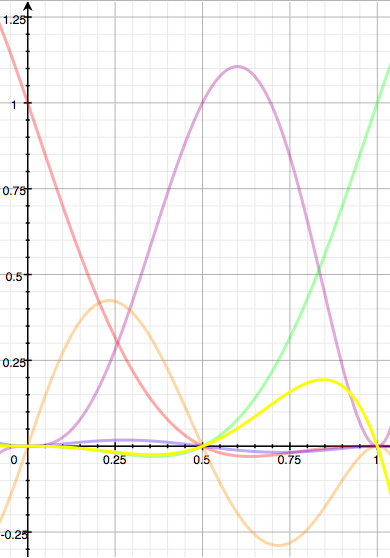
\includegraphics{basis-graph}

2. Find a matrix $M$ such that if $P_{Bez} = MP_{Bsp}$, then $f_{Bez}(u) = f_{Bsp}(u) \forall u$. 

$$f_{Bsp}(u) = 
\begin{bmatrix}
1 &
u &
u^2 &
u^3
\end{bmatrix}
\frac{1}{6}
\begin{bmatrix}
-1 & 3 & -3 & 1 \\
3 & -6 & 3 & 0 \\
-3 & 0 & 3 & 0 \\
1 & 4 & 1 & 0 
\end{bmatrix}
P_{Bsp}
$$

$$f_{Bez}(u) = 
\begin{bmatrix}
1 &
u &
u^2 &
u^3
\end{bmatrix}
\begin{bmatrix}
-1 & 3 & -3 & 1 \\
3 & -6 & 3 & 0 \\
-3 & 3 & 0 & 0 \\
1 & 0 & 0 & 0 
\end{bmatrix}
P_{Bez}
$$

So given that we have $f_{Bsp}(u) = \vec{u}\frac{1}{6}M_{Bsp}P_{Bsp}$ and $f_{Bez}(u) = \vec{u}M_{Bez}P_{Bez}$, we substitute as $f_{Bez}(u) = f_{Bsp}(u) = \vec{u}M_{Bez}MP_{Bsp}$

Now we can isolate $M_{Bez}M = \frac{1}{6}M_{Bsp}$ and solve for $M = M_{Bez}^{-1}\frac{1}{6}M_{Bsp}$

\begin{align*}
M &= 
\begin{bmatrix}
-1 & 3 & -3 & 1 \\
3 & -6 & 3 & 0 \\
-3 & 3 & 0 & 0 \\
1 & 0 & 0 & 0 
\end{bmatrix}^{-1}
\frac{1}{6}
\begin{bmatrix}
-1 & 3 & -3 & 1 \\
3 & -6 & 3 & 0 \\
-3 & 0 & 3 & 0 \\
1 & 4 & 1 & 0 
\end{bmatrix}
\\
M &= 
\frac{1}{6}
\begin{bmatrix}
0 & 0 & 0 & 1 \\
0 & 0 & \frac{1}{3} & 1 \\
0 & \frac{1}{3} & \frac{2}{3} & 1 \\
1 & 1 & 1 & 1
\end{bmatrix}
\begin{bmatrix}
-1 & 3 & -3 & 1 \\
3 & -6 & 3 & 0 \\
-3 & 0 & 3 & 0 \\
1 & 4 & 1 & 0 
\end{bmatrix}
\\
M &= 
\frac{1}{6}
\begin{bmatrix}
1 & 4 & 1 & 0 \\
0 & 4 & 2 & 0 \\
0 & 2 & 4 & 0 \\
0 & 1 & 4 & 1
\end{bmatrix}
\end{align*}

b. The graph is as follows, with the blue for b-Spline points and the red for converted Bezier points. 

 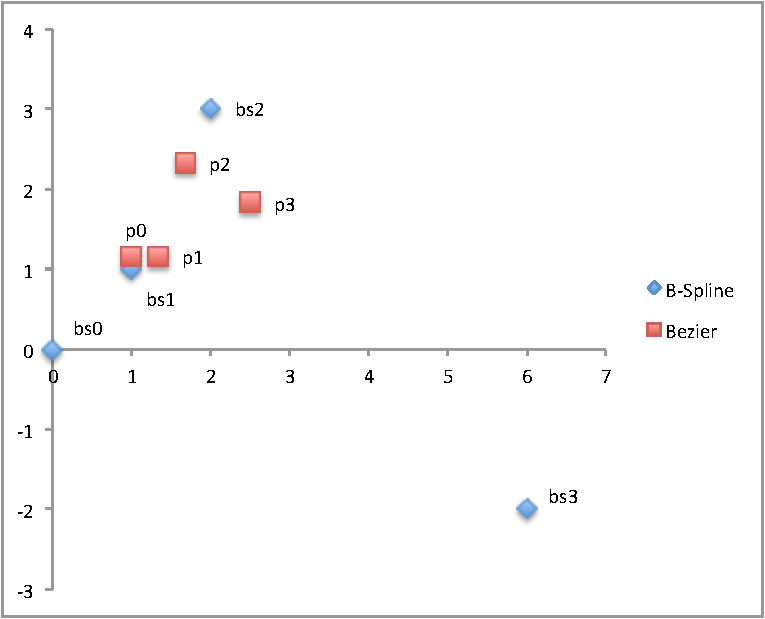
\includegraphics{bezier-plot4}
 
 % [width=400pt]

\end{document}